\section{Постановка задачи и описание данных} \label{section:task}

\subsection{Неформальная постановка задачи}
Пусть имеется выборка трехмерных обектов, представленных в виде облаков точек (point clouds). Необходимо создать алгоритм, который на основе данной выборки будет генерировать \textit{новые} объекты подобные объектам в выборке, то есть будет генерировать новые объекты с сохранением статистических и геометрических свойств исходных объектов.

\subsection{Формальная постановка задачи}

\subsection{Описание данных}

В данной работе, поставленная задача решается на основе выборки зубов человека.

Опишем некоторые термины и понятия из зубного дела.

\subsubsection{Зубная анатомия}

Зубы классифицируются на резцы (incisors), клыки (canines), премоляры (premolars) и моляры (molars). Вместе зубы объединяются в верхний и нижний зубные ряды. Каждая зубная дуга (dental arch), или по-другому ряд зубов, разделяется на левую и правую часть. С каждой стороны у человека имеется два резца, один клык, два премоляра и три моляра \cite{kumar}.

\begin{figure}[h]
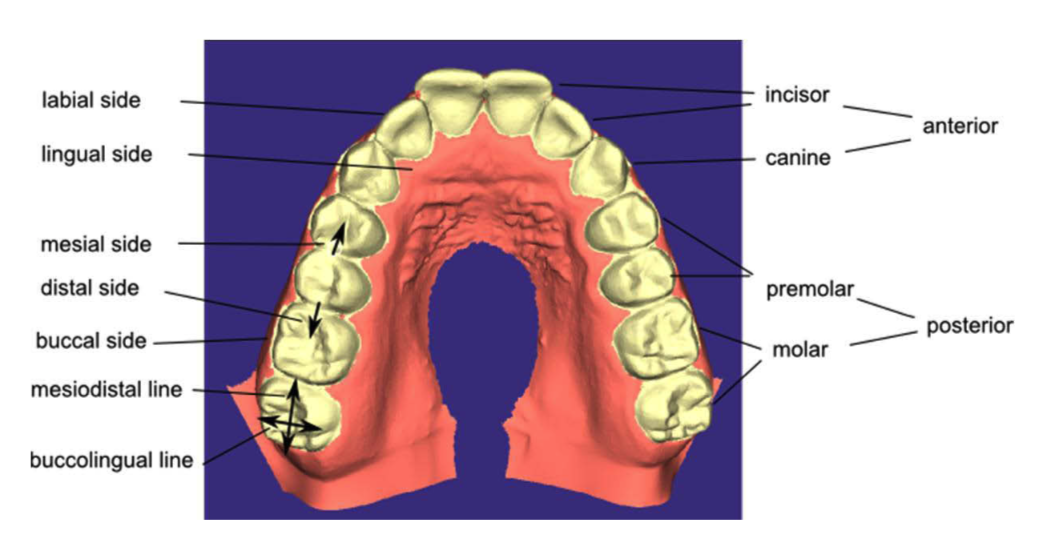
\includegraphics[width=1\linewidth]{images/dental_parts.png}
\caption{Анатомия зубов}
\label{fig:dental_parts}
\end{figure}

% ls | grep -e "^[0-9]" | while read dir; do ls $dir | nl | tail -n1; done

\subsubsection{Размер выборки}

В выборке присутствуют 28 типов зубов (все, кроме третьих моляров - зубов мудрости), для каждого типа зуба имеется от 124 до 150 экземпляров. Все экземпляры представлены в виде трехмерных сеток (перед началом работы основного алгоритма мы переводим их в облака точек, путем отбрасывания ребер). Примеры экземпляров из выборки можно увидеть на  изображениях:


\begin{figure}[h]
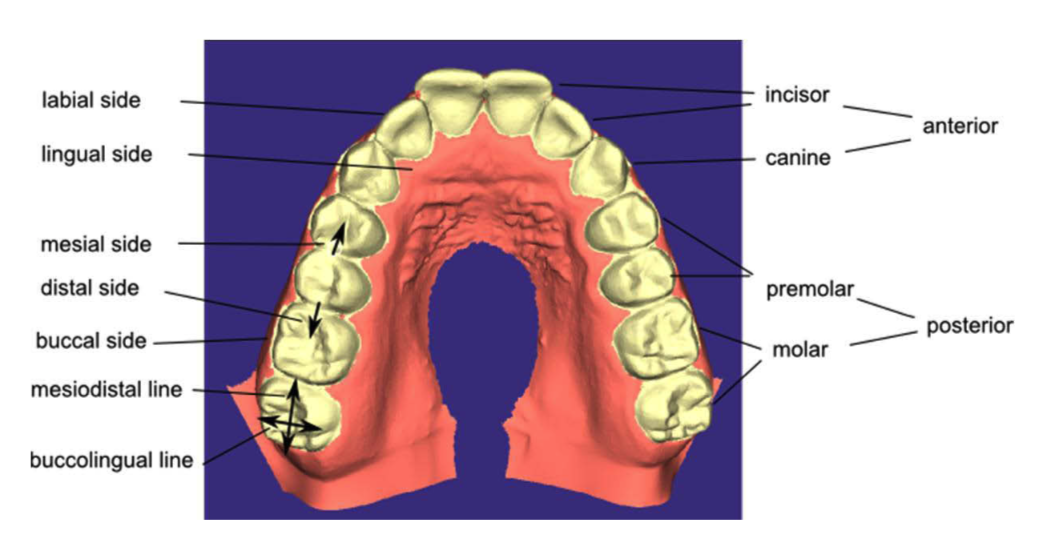
\includegraphics[width=1\linewidth]{images/dental_parts.png}
\caption{Анатомия зубов}
\label{fig:tooth_1}
\end{figure}


\begin{figure}[h]
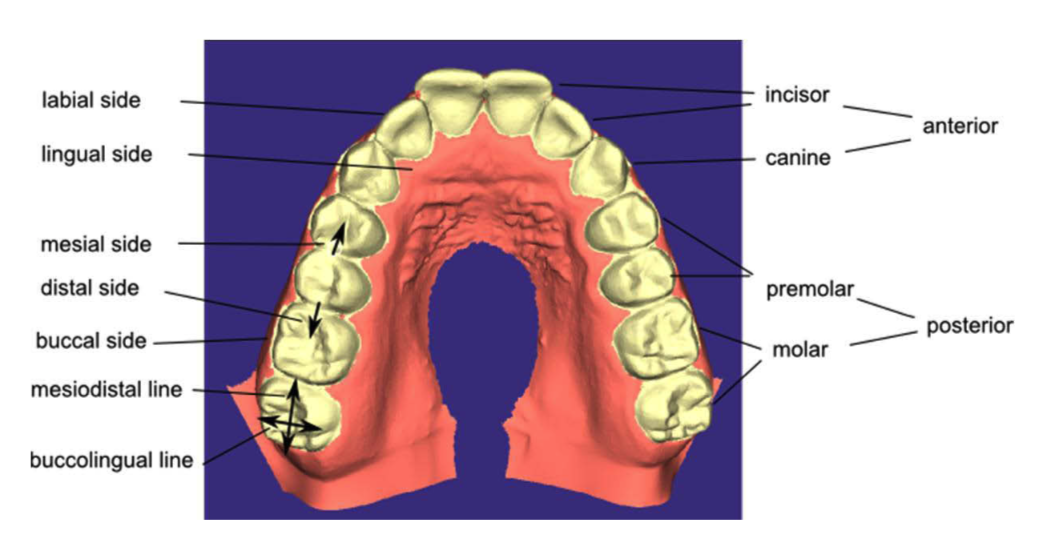
\includegraphics[width=1\linewidth]{images/dental_parts.png}
\caption{Анатомия зубов}
\label{fig:tooth_2}
\end{figure}


\begin{figure}[h]
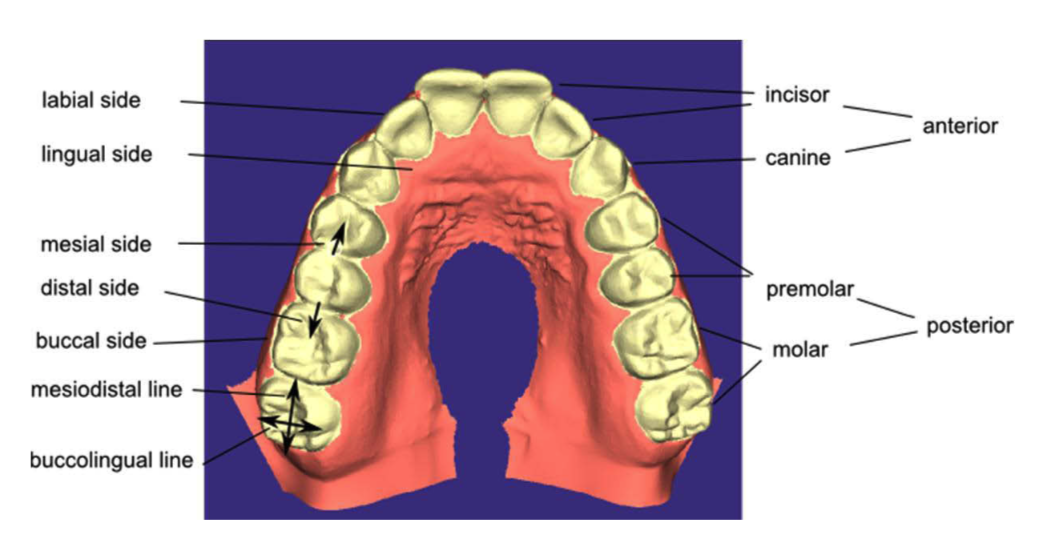
\includegraphics[width=1\linewidth]{images/dental_parts.png}
\caption{Анатомия зубов}
\label{fig:tooth_3}
\end{figure}